\chapter{Baggrund For Projektet}
\label{Background}
\section{Udfordringen ved et bookingsystem}
\label{Baggrund_Udfording}
I lang tid har lokale bookning på ITU været et uoverskueligt og problemfyldt område, der har forhindret at ITU's lokaler kunne bruges optimalt. Vi vurderer derfor, at det er vigtigt at udvikle et ordentligt lokale bookingsystem således, at ITU kan udnytte deres mange lokaler optimalt.

 Det udfordrende ved et bookingsystem er, at det er et servicesystem, der både skal understøtte servicer til booking af lokaler samt opdatering og vedligeholdelse af systemet. Der er derfor mange aktører og mange arbejdsområder der skal tages hensyn til.

 For at have overblik over, hvad der skulle understøttes og hvad der var vigtigst fulgte vi en kravspecifikation som blev udarbejdet i kurset "Anskaffelse og kravspecifikation" på ITU i efteråret 2012. Kravspecifikationen er lavet med fokus specifikt på ITU og hvad et bookingsystem til ITU kræver.
\section{Kravspecifikationen og ændringer}
\label{Baggrund_kravspecifikationen}
I kravspecifikationen beskrives hvordan den nuværende booking situation er på ITU, i øjeblikket foregår bookingen af lokaler i mange forskellige systemer, hvor der er en aktør som fungerer som bindeled for administrationen af lokaler. For at forbedre den løsning foreslår kravspecifikationen, at der laves et system som alle aktørerne arbejder op imod. Det er så vidt muligt den løsning vi vil lave en begrænset implementering af. Figur \ref{} viser den nuværende situation.

\begin{figure}[h!]
  \centering
    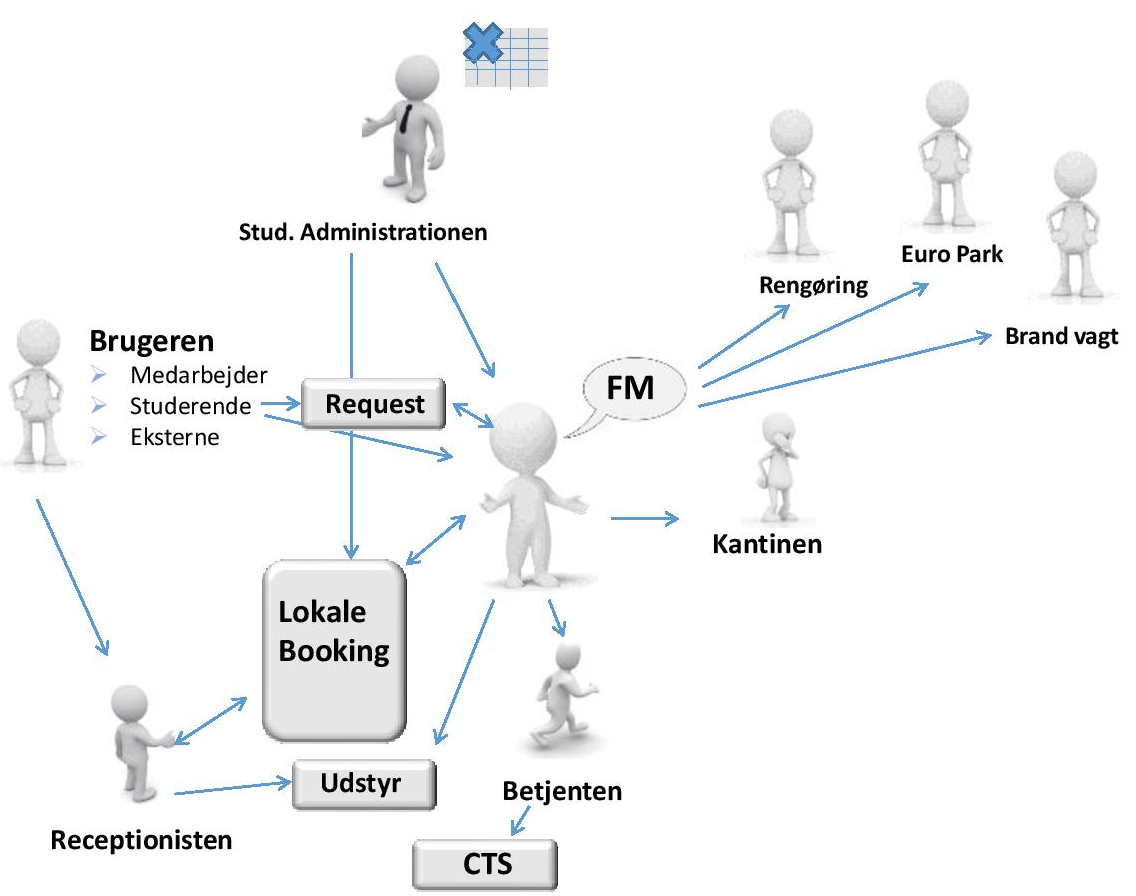
\includegraphics[width=0.5\textwidth]{Appendix/GUI-Prototype/NuvaerendeFlow}
  \caption{Nuværende system flow for booking systemet på ITU}
\label{Baggrund_kravspecifikationen_NuvaerendeFlow}
\end{figure}

\subsection{Ændringer til kravspecifikationen}
\label{Baggrund_kravspecifikationen_Aendringer}
Kravspecifikationen præsenterer en datamodel, der beskriver hvilke informationer systemet skal bruge. Vi har lavet nogle ændringer så den passer til vores implementering af bookingsystemet. Vi har fjernet lokale status og lavet en ”mange til én” forbindelse mellem booking og lokale da vi gerne ville have, at en booking kun kunne have et lokale.

 Vi fjernede også "Lokale egenskaber" da vi vurderede, at det gav mest mening hvis "Inventar" repræsenterede et unikt stykke inventar og ikke havde antal i "Lokale egenskaber". Vi slettede også alle ”pris” værdier fra modellen, da vi ikke havde nogen intention om at understøtte fakturering.
\section{Arbejdsopgaver}
\label{Baggrund_Arb_opgaver}
Denne sektion beskriver hvilke arbejdsopgaver vi understøtter i første release samt giver en prioritering af, hvilke arbejdsopgaver der bør fokuseres på i følgende releases.
\subsection{Arbejdsområde 1: Booking}
\label{Baggrund_Arb_opgaver_Booking}
\subsubsection{C1: Administrer booking}
\begin{tabular}{ | l | r | p{5} |}
	\hline
	Arbejdesopgave & \\ 
\hline
	C1.1 & Understøttet \\ 
\hline
	C1.1a & Understøttet \\ 
\hline
	C1.2 & Understøtet \\ 
\hline
	C1.2a & Understøttet \\ 
\hline
	C1.3 & Understøttet \\ 
\hline
	C1.4 & Understøttet \\ 
\hline
	C1.5 & Understøttet \\ 
\hline
\end{tabular}

\subsubsection{C2: Forespørg på booking}
\begin{tabular}{ | l | r | p{5} |}
	\hline
	Arbejdesopgave & \\ 
\hline
	C2.1 & Understøttet \\ 
\hline
	C2.1a & Understøttet \\ 
\hline
	C2.2 & Understøttet \\ 
\hline
	C2.3 & Understøttet \\ 
\hline
\end{tabular}

\subsection{Arbejdsområde 2: Booking behandling}
\label{Baggrund_Arb_opgaver_Booking_behandling}
\subsubsection{C3: Modtag forespørgsel fra Eksern}
\begin{tabular}{ | l | r | p{5} |}
	\hline
	Arbejdesopgave & \\ 
\hline
	C3.1 & Understøttet \\ 
\hline
	C3.2 & Understøttet \\ 
\hline
	C3.2a & Understøttet \\ 
\hline
	C3.3 & Ikke understøttet \\ 
\hline
	C3.4 & Understøttet \\ 
\hline
	C3.5 & Understøttet \\ 
\hline
	C3.6 & Ikke understøttet \\ 
\hline
\end{tabular}

\subsubsection{C4: Klargør lokaler}
\begin{tabular}{ | l | r | p{5} |}
	\hline
	Arbejdesopgave &\\ 
\hline
	C4.1 & Ikke understøttet \\ 
\hline
	C4.2 & Ikke understøttet \\ 
\hline
	C4.3 & Ikke understøttet \\ 
\hline
\end{tabular}

\subsubsection{C5: Udlever nøgle}
\begin{tabular}{ | l | r | p{5} |}
	\hline
	Arbejdesopgave & \\ 
\hline
	C5.1 & Ikke understøttet \\ 
\hline
	C5.2 & Ikke understøttet \\ 
\hline
\end{tabular}

\subsection{Arbejdsområde 3: Forplejning}
\label{Baggrund_Arb_opgaver_Forplejning}
\subsubsection{C6: Håndter forplejning}
\begin{tabular}{ | l | r | p{5} |}
	\hline
	Arbejdesopgave & \\ 
\hline
	C6.1 & Ikke understøttet \\ 
\hline
	C6.2 & Ikke understøttet \\ 
\hline
	C6.3 & Ikke understøttet \\ 
\hline
	C6.4 & Ikke understøttet \\ 
\hline
\end{tabular}

\subsubsection{C7: Fakturer forplejning}
\begin{tabular}{ | l | r | p{5} |}
	\hline
	Arbejdesopgave & \\ 
\hline
	C7.1 & Ikke understøttet \\ 
\hline
	C7.5 & Ikke understøttet \\ 
\hline
\end{tabular}

\subsubsection{C8: Opadter menukort}
\begin{tabular}{ | l | r | p{5} |}
	\hline
	Arbejdesopgave & \\ 
\hline
	C8.1 & Ikke understøttet \\ 
\hline
\end{tabular}

\subsection{Arbejdsområde 3: Systemadministration}
\label{Baggrund_Arb_opgaver_Systemadmin}
\subsubsection{C9: Opdater listen for ekstra udstyr}
\begin{tabular}{ | l | r | p{5} |}
	\hline
	Arbejdesopgave & \\ 
\hline
	C9.1 & Understøttet \\ 
\hline
\end{tabular}

\subsubsection{C10: Opdater lokaler}
\begin{tabular}{ | l | r | p{5} |}
	\hline
	Arbejdesopgave & \\ 
\hline
	C10.1 & Understøttet \\ 
\hline
	C10.2 & Understøttet \\ 
\hline
\end{tabular}

\subsubsection{C11: Administrer bruger}
\begin{tabular}{ | l | r | p{5} |}
	\hline
	Arbejdesopgave & \\ 
\hline
	C11.1 & Ikke understøttet \\ 
\hline
	C11.1a & Ikke understøttet \\ 
\hline
\end{tabular}

\subsubsection{C12: Håndter statistik}
\begin{tabular}{ | l | r | p{5} |}
	\hline
	Arbejdesopgave & \\ 
\hline
	C12.1 & Ikke understøttet \\ 
\hline
	C12.2 & Ikke understøttet \\ 
\hline
\end{tabular}

\subsection{Arbejdsområde 4: Finans}
\label{Baggrund_Arb_opgaver_Finas}
\subsubsection{C13: Behandel faktura}
\begin{tabular}{ | l | r | p{5} |}
	\hline
	Arbejdesopgave & \\ 
\hline
	C13.1 & Ikke understøttet \\ 
\hline
	C13.2 & Ikke understøttet \\ 
\hline
\end{tabular}
\subsection{Prioritering af arbejdsopgaver}
\label{Baggrund_Arb_opgaver_Prio_Arb_Opg}
Til den første release af systemet valgte vi at fokusere på at understøtte systemadministration og booking af lokaler og udstyr, hvilket tydeligt kan ses i afsnit\ref{Baggrund_Arb_opgaver} da alle arbejdsopgaver i arbejdsområderne C1,C2,C3,C9 og C10 er understøttet. I

 kravspecifikationen er de arbejdsområder også blandt dem som er vægtet højest og det er samtidig de arbejdsområder som indeholder kernefunktionerne i systemet. Det som ikke blev prioriteret højt nok til at komme med i første release var de arbejdsopgaver som fokuserede på integrationen med kantinen, samt mulighed for fakturing og statestik , arbejdsopgaverne C6.1- C6.4, C12.1- C12.2 er eksempler på sådanne opgaver.
\\Grunden til at vi ikke tog de arbejdsopgaver med var, at vi vurderede, at de ikke var nødvendige for at have et system der understøttede basis funktioner, derudover lagde arbejdsopgaverne op til, at der skulle implementeres et interface specifikt til kantinen hvilket vi vurderede ville tage lang tid at implementere og vi ville også have tre brugergrupper at tage hensyn til ift. usability og testing.
\\Fokus for næste release vil derfor være at få udarbejdet et interface som kantinen kan bruge til at integrere med resten af systemet og få finpudset de allerede eksisterende funktioner i kravspecifikationen. Behandling af faktura har også en høj vægtning, så det vil der også blive lagt fokus på. 
